%!TEX root = ../../../thesis.tex
\section{Current Trends in Water Metering}
  Automatic meter reading systems offer advantages to suppliers of town water.
  These include increased billing frequency, remove the need to access the consumers' property~\cite{Chang2012}, and help reduce overall water consumption.
  Another factor in the adoption automatic meter reading technologies is the ability to detect water leaks.
  It has been estimated that as much as \SI{10}{\percent} of post-meter water consumption is due to leakage in the residential sector.
  A study by Britton et al.\ found that by communicating with those customers whose water supply exhibited signs of leakages, a total reduction of  \SI{89}{\percent} of night-time flow rates was achieved.
  This is in contrast to a control group whose night-time usage increased by over \SI{50}{\percent}.
  In areas where water availability is limited, conserving water is an important issue.
  The benefits of automatic water metering are not only geared toward fair pricing but detecting and monitoring the network as a whole.

  \begin{figure}
    \centering
    \includegraphics[width=0.9\textwidth]{content/pt1/02-WirelessWaterMeter/graphics/meter}
    \caption{\label{fig:Photo_DomesticWaterMeter}Photograph of a domestic water meter (Kent PSMT 25mm) typically found in the Auckland region.}
  \end{figure}

  Domestic water meters are typically placed at a property's boundary in a plastic box set into the ground.
  The meter at my Auckland home is shown as \cref{fig:Photo_DomesticWaterMeter}.
  This is a typical meter for the Auckland region, which has been installed approximately eight meters into our property from the road-side.
  Due to their location, it is usually not feasible to wire them to an electrical grid.
  No commercially viable domestic energy harvesting water meters, suitable for burial, exist on the market as of writing.

  \begin{figure}
    \centering
    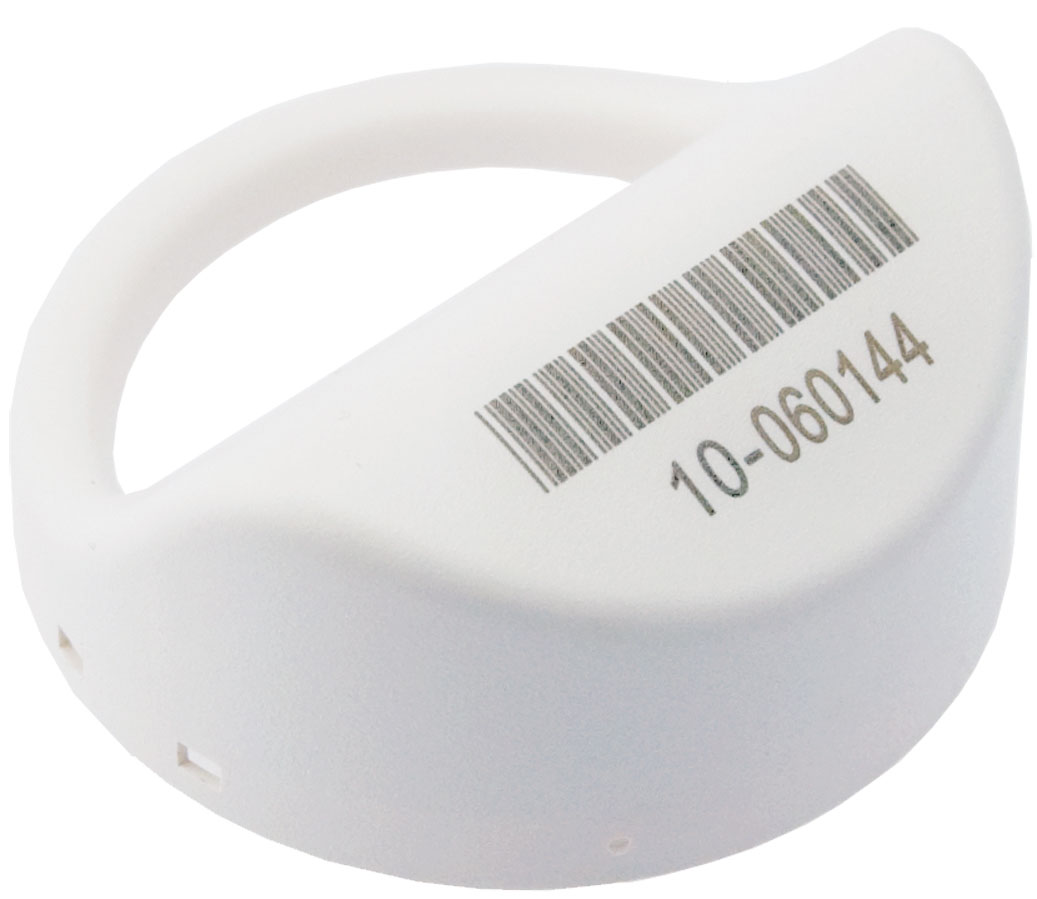
\includegraphics[width=0.5\textwidth]{content/pt1/02-WirelessWaterMeter/graphics/hydro-WMBUSWLESSM}
    \caption{\label{fig:Photo_waterwareMeter}Photograph of the a wireless transmitting module from Waterware NZ. The device clips onto a compatable water meter and contains its own battery~\cite{BMeters2014}.}
  \end{figure}

  A common configuration for wireless automatic meter reading is to have a reader/transmitter device that is separate to the meter itself.
  This allows new businesses to enter the remote metering market without having to develop metering technologies.
  Such a device may sit on the meter's display or have a wire that connects it to the meter.
  The design; being a simple tamper-proof, clip-on device; means that it must be powered by batteries.

  Current automatic meter reading systems employ long-life, non-rechargeable batteries.
  These meter reading systems have a battery life of around ten years~\cite{BMeters2014}, which is near the shelf-life of the battery itself.
  We want to see if streaming cells could be used as a means to provide sufficient energy to monitor water usage.
  If possible, a suitable harvester would remove the need for batteries, but require plumbing into the domestic feed.
  The resulting device would not be an attachment, but a replacement for the traditional water meter.
  This would mean that it would have to take on the role of metering water usage.


\section{Appropriateness of Streaming Cell Harvesters}

  In \cref{chap:harvestingEnergy} we discussed electric power generation from streaming cells.
  I demonstrated a \SI{0.2}{\micro\percent} conversion efficency from water flow and pressure.
  I also found the streaming voltage is directly proportional to the pressure across a cell.
  Can that pressure dependence give a way to meter water consumption while generating power? Probably.
  But that sort of question is only relevant if the harvester is feasible.

  To find that out - we need to know how much energy is available to an energy harvester.


  \subsection{Readily harvestable energy}
    This section determines the amount of enery available to an energy harvester.
    The harvester envisioned is intended for domestic water metering so we start by building a profile of domestic water consumption.
    Then by finding how much energy is lost inside a typical water meter we will know how much energy a harvester has available.

    \begin{table}
      \centering
      \begin{tabular}{r l|r|r|l}
        Item & Measurement & Summer & Winter & Unit\\
        \hline\hline
        \multirow{4}{*}{Shower} & Duration & 6.6 & 7.0 & minutes\\
                                & Volume & 50.0 & 52.5 & litres\\
                                & Flow & 8.1 & 8.0 & litres/minute\\
                                & Frequency & 0.9 & 0.9 & /person/day\\
        \hline
        \multirow{2}{*}{Washing}& Volume & 122 & 123 & litres\\
                                & Frequency & 0.35 & 0.36 & /person/day\\
        \hline
        \multirow{2}{*}{Toilet} & Volume & 6.6 & 6.8 & litres\\
                                & Frequency & 4.9 & 4.5 & /person/day\\
      \end{tabular}
      \caption{\label{tab:consumption_figures}Summary of characteristics for typical toilet usage, data taken from~\cite{Heinrich2008}.}
    \end{table}

    In 2008, Heinrich monitors water consumption of 51 homes throughout Auckland in 2008~\cite{Heinrich2008}.
    The report shows that the majority of domestic water is consumed by the shower (\SI{30}{\percent}), washing machine (\SI{27}{\percent}) and toilet (\SI{20}{\percent}).
    Together these account for over \SI{75}{\percent} of domestic water consumption.
    Data shown in \cref{tab:consumption_figures} was taken from that report in order to build a typical water usage profile.
    In 2007, Heinrich published a similar report which also contained water flow profiles~\cite{Heinrich2007} for each of the three items considered.

    \begin{figure}
      \centering
      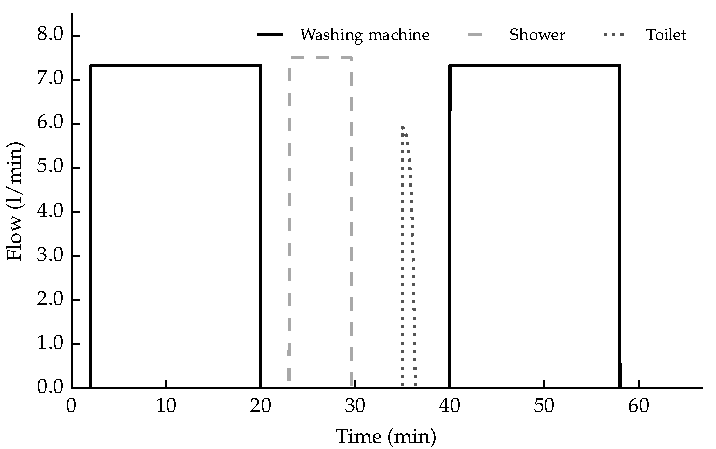
\includegraphics[width=\linewidth]{content/pt1/02-WirelessWaterMeter/graphics/graph_profile}
      \caption{Sample profile showing constructed instances of washing machine use, a shower and a toilet flush.
      Washing machine usage is broken into two parts corresponding to a wash and rinse cycle.}
      \label{fig:profileSample}
    \end{figure}

    Data from those reports has been used to build a domestic water usage profile.
    \Cref{fig:profileSample} shows the flow rates for each of the items
    The profile fits the usage statistics of a home with two occupants according to the previously mentioned reports over the duration of a week.

    During that time five uses of a washing machine, fourteen showers and fifty six toilet flushes occur.
    \Cref{fig:profileSample} shows
    A sample of the usage profiles of each item is shown in Fig. \ref{fig:profileSample}.

    \begin{figure}
        \centering
        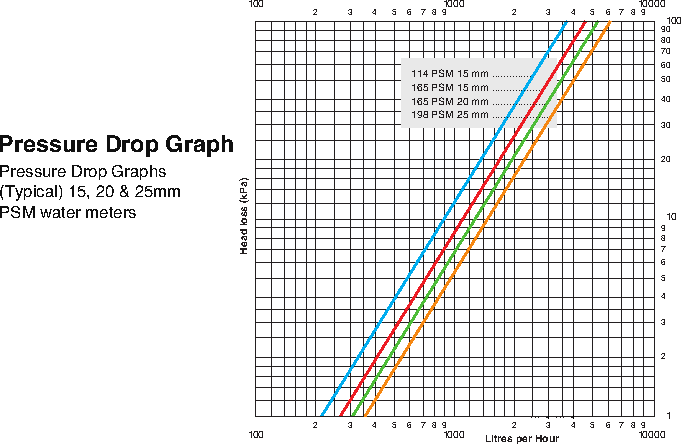
\includegraphics[width=\linewidth]{content/pt1/02-WirelessWaterMeter/graphics/Kent-PSM-HeadLoss}
        \caption{Graph showing the pressure developed across the Kent PSM series mechanical water meters. Taken from~\cite{Elster2008}.}
        \label{fig:headloss}
    \end{figure}

    \begin{figure}
        \centering
        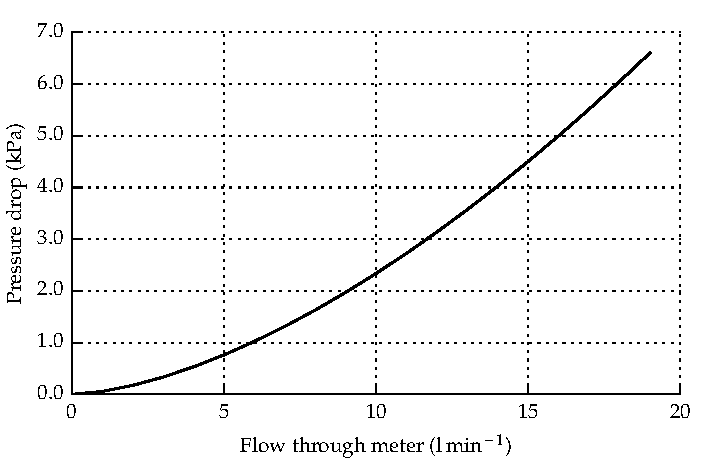
\includegraphics[width=\linewidth]{content/pt1/02-WirelessWaterMeter/graphics/graph_pressureLoss}
        \caption{Graph showing fitted curve to the pressure loss graph presented as \cref{fig:headloss}.}
        \label{fig:headloss_fit}
    \end{figure}

    \begin{figure}
        \centering
        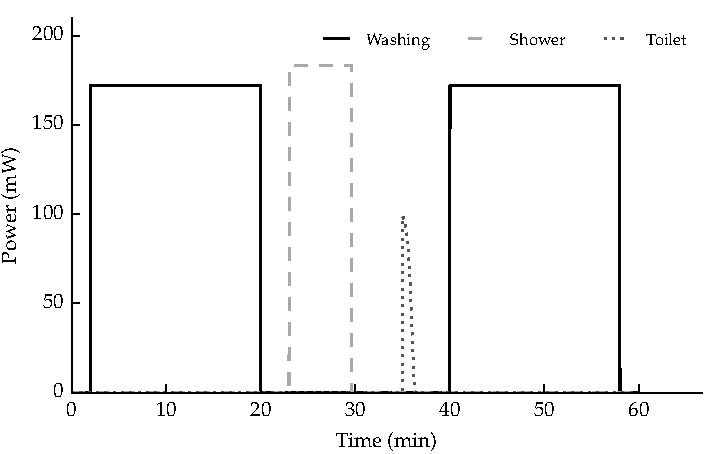
\includegraphics[width=\linewidth]{content/pt1/02-WirelessWaterMeter/graphics/graph_harvest}
        \caption{Calculated power dissipation by a typical domestic mechanical water meter for each of the sample profile events.}
        \label{fig:powerDissipated_meter}
    \end{figure}

    Fig.~\ref{fig:headloss} shows the pressure head loss curve from a water meter typically installed at New Zealand homes (Kent PSMT 25mm)~\cite{WatercareNewZealand2014}.

    Using this curve we calculate power dissipation in a water meter during a washing machine cycle, shower, and toilet flush; presented as \cref{fig:powerDissipated_meter}.
    The total energy dissipated within the meter for each events is:
    \begin{itemize}
    \item \SI{547}{\joule} per load of washing,
    \item \SI{222}{\joule} per shower, and
    \item \SI{24.3}{\joule} per flush of the toilet.
    \end{itemize}

% washing machine volume = 122.00 l
% shower volume = 49.50 l
% toilet volume = 6.22 l
% washing machine energy = 172.08 l
% shower energy = 72.62 l
% toilet energy = 5.07 l

    % These figures are based on average duration and flow rates as found in \cite{Heinrich2008}, and the estimated head loss from Fig.~\ref{fig:headloss}.
    Over an average week the reference water meter would dissipate approximately \SI{7.20}{\kilo\joule} of energy; averaging \SI{1.03}{\kilo\joule} per day.


  \subsection{Domestic harvester design}



    \begin{figure}
      \centering
      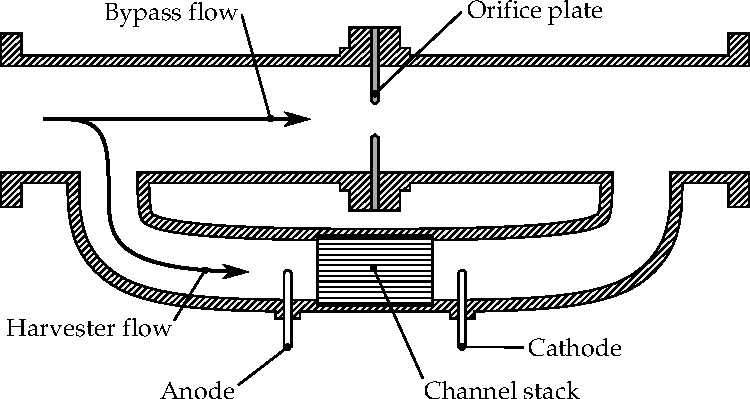
\includegraphics[width=0.9\textwidth]{content/pt1/02-WirelessWaterMeter/graphics/harvester}
      \caption{\label{fig:Diagram_harvester}Diagram showing the intended design of streaming cell harvester suitable for domestic connection.}
    \end{figure}